% ==============================================================================
% Section 2: Key Findings
% ==============================================================================

\section{Key Findings}
\label{sec:key_findings}

\subsection{The universal crash: no scenario averts catastrophic decline}
\label{sec:findings_crash}

The single most important result of this study is sobering: under every scenario we
tested, \textit{Pycnopodia helianthoides} populations collapse to roughly 5\% of their
historical peak by 2050 (Figure~\ref{fig:coastwide_population}). The baseline
scenario (F01: moderate warming, full pathogen evolution) yields 238,687 surviving
individuals---5.4\% of the peak population of 4,447,241. Disabling all pathogen
evolution (F02) improves this only marginally, to 261,632 individuals (5.9\%).
Allowing thermal adaptation but blocking virulence evolution (F03) produces the
worst outcome at 224,638 individuals (5.1\%). Even the high-warming scenario (F04)
lands at 258,760 individuals (5.8\%), virtually indistinguishable from the baseline
at the coastwide scale.

The narrow range of these outcomes---5.1\% to 5.9\%---demands attention. Neither the
climate trajectory nor the pathogen's evolutionary capacity meaningfully alters the
coastwide picture. The total difference between the best and worst scenarios amounts
to approximately 37,000 individuals out of a pre-epidemic population of nearly 4.5
million. This is not a system where optimistic assumptions buy substantially better
outcomes. The disease has fundamentally restructured \textit{Pycnopodia} populations,
and recovery to anything resembling historical abundances does not occur within
the forecast horizon under any scenario we examined.

This result should anchor all subsequent conservation planning: natural recovery
alone will not restore \textit{Pycnopodia} to ecological functionality by mid-century.
Active intervention---captive breeding, reintroduction, habitat management---is not
optional; it is the only pathway to meaningful recovery on management-relevant
timescales.

% --- Figure: Coast-wide Population Trajectories ---
\begin{figure}[!htbp]
    \centering
    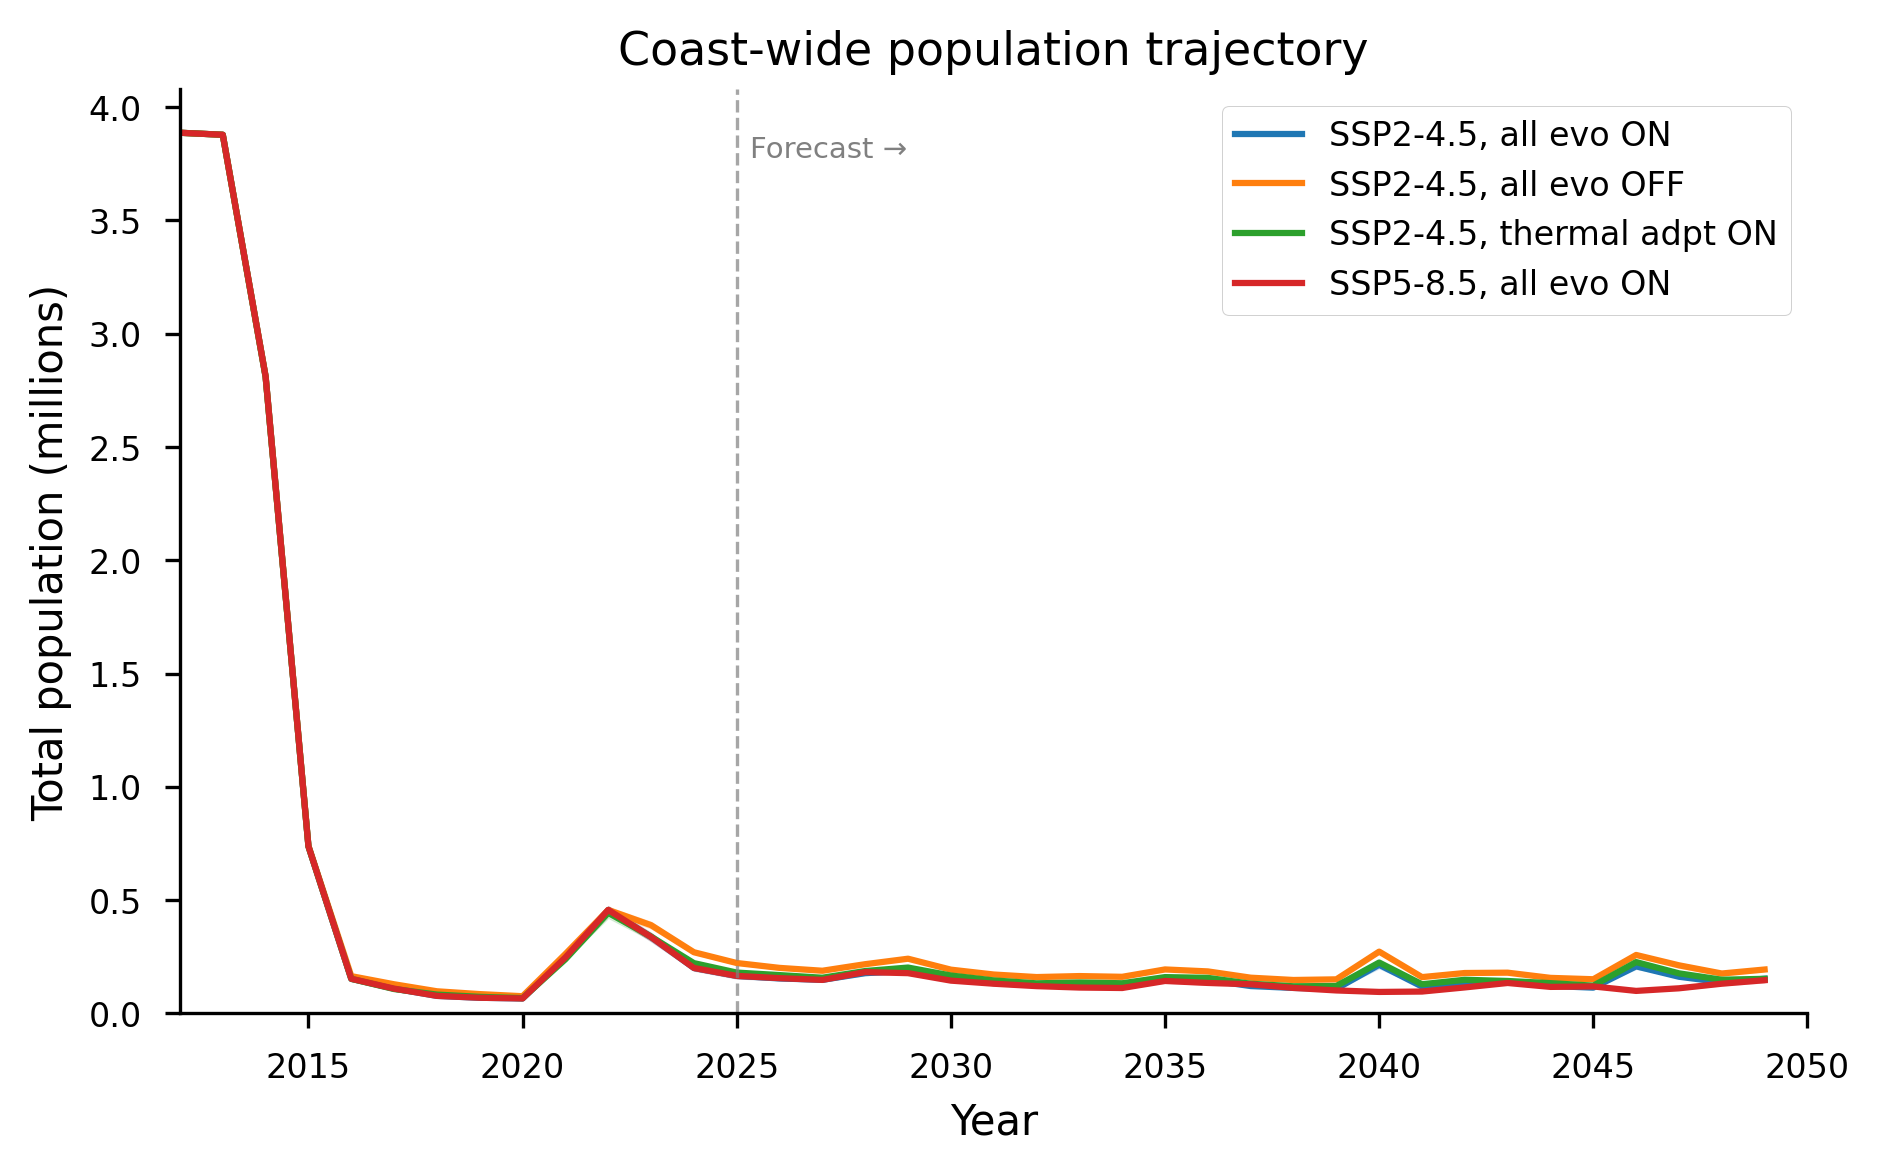
\includegraphics[width=0.85\textwidth]{figures/fig_coastwide_population.png}
    \caption{Coast-wide \textit{Pycnopodia helianthoides} population trajectories under four forecast scenarios (2012--2050). Solid lines show three-seed means; shaded bands indicate $\pm$1 standard deviation. The vertical dashed line at 2025 marks the transition from observed SST (NOAA OISST) to projected SST (CMIP6 delta method). All scenarios show a catastrophic crash in 2013--2015 followed by intermittent recovery attempts and long-term stabilization at approximately 5\% of peak abundance. The narrow spread among scenarios (5.1--5.9\% surviving) indicates that the coastwide outcome is robust to both climate pathway and evolutionary assumptions.}
    \label{fig:coastwide_population}
\end{figure}

\subsection{The Oregon surprise: geography of survival}
\label{sec:findings_oregon}

Although the coastwide numbers are uniformly grim, the regional picture reveals
striking heterogeneity (Figure~\ref{fig:regional_recovery_bars}). Under the
baseline scenario (F01), Alaska's Fairweather-North region (AK-FN) retains the 
highest fraction of its peak population at 6.8\%, followed by Oregon at 5.4\% 
(5-year average, see endpoint bias discussion below). Central California follows at 11.9\%, then outer Washington
coast at 8.8\%, the Fairweather--Yakutat coast of Alaska (AK-FN) at 6.8\%, and
the southern Salish Sea (SS-S) at 6.5\%.

% --- Figure: Regional Recovery Bars ---
\begin{figure}[!htbp]
    \centering
    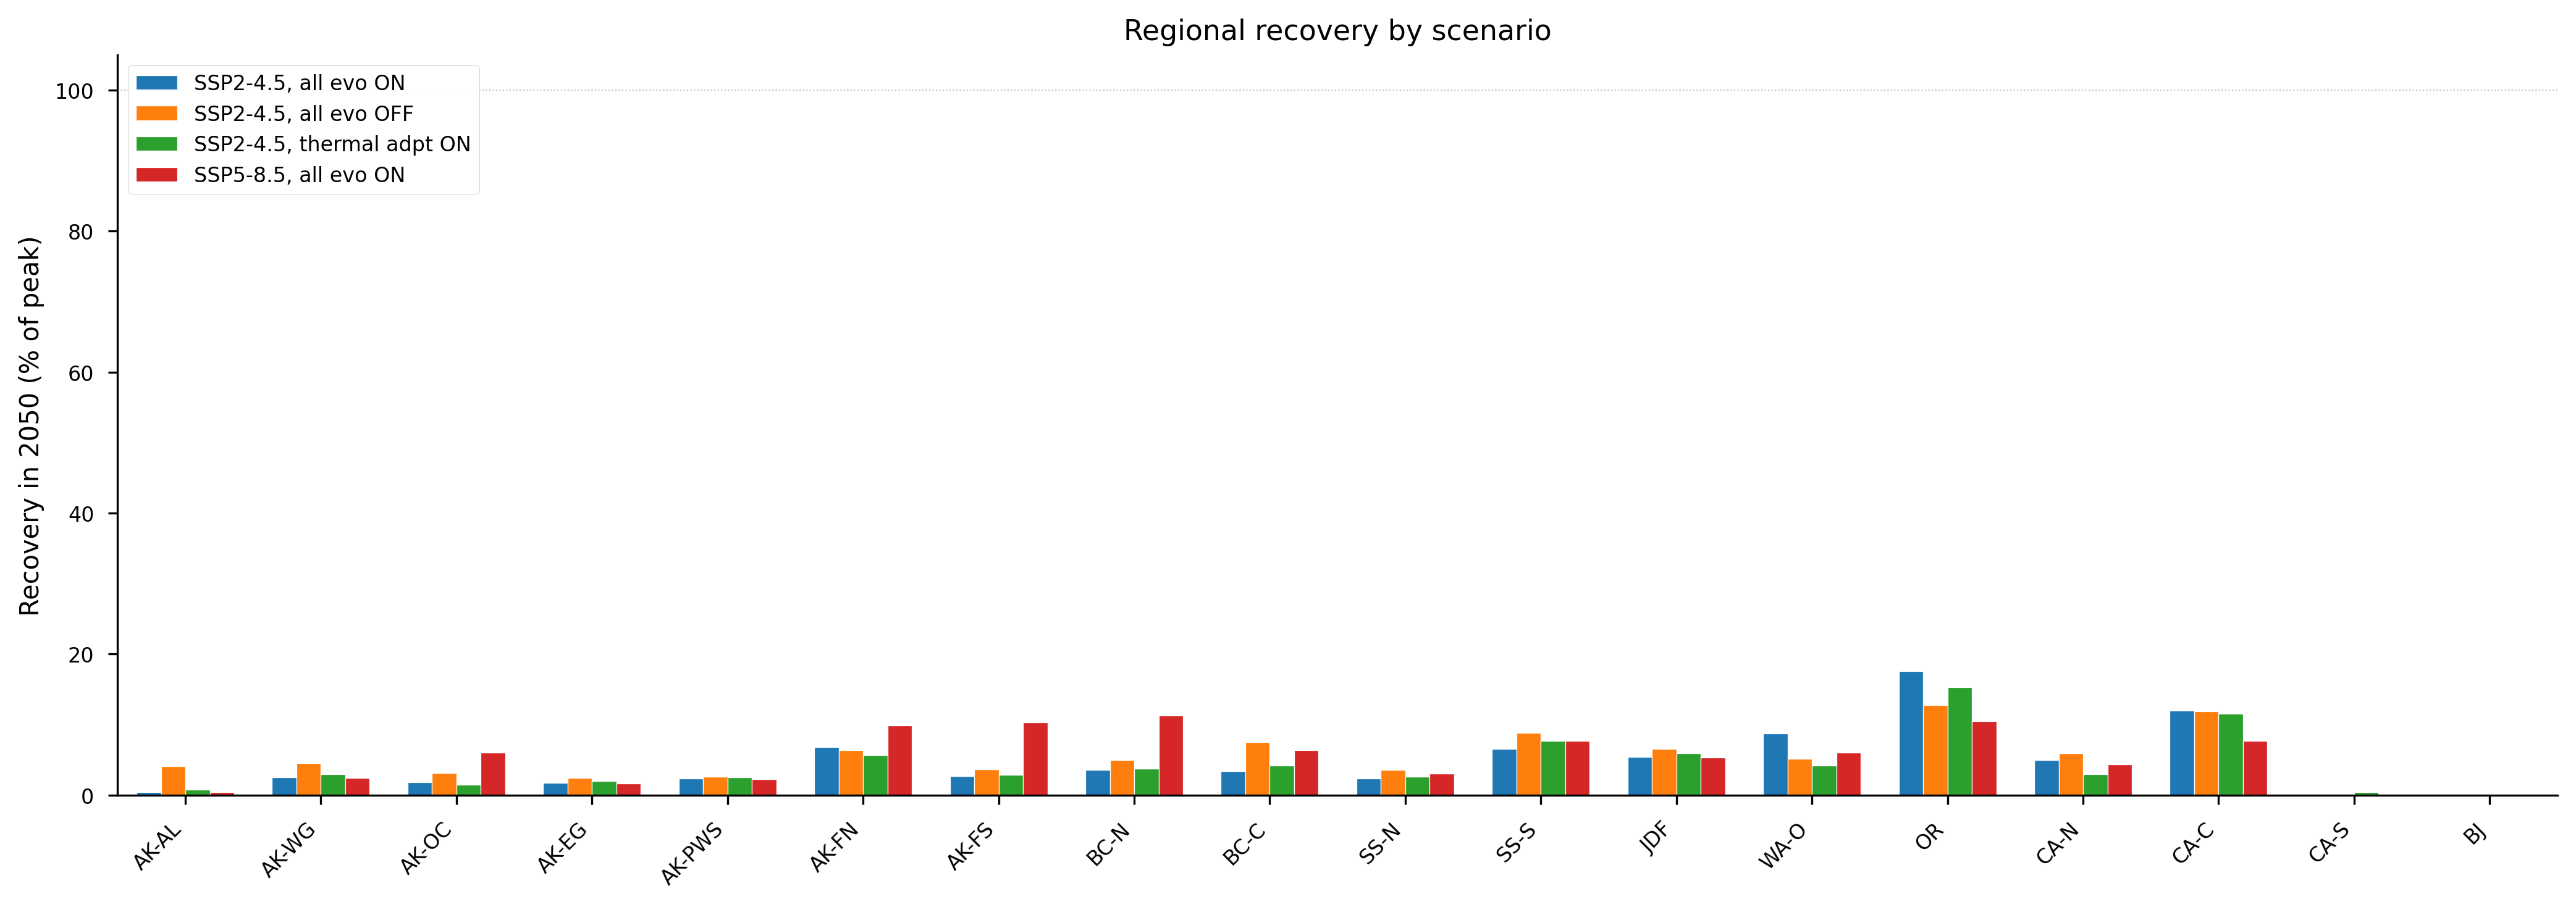
\includegraphics[width=\textwidth]{figures/fig_regional_recovery_bars.png}
    \caption{Regional recovery as a percentage of pre-disease peak population, by scenario. Regions are ordered from north (left) to south (right). Alaska's Fairweather-North (AK-FN) shows the most reliable recovery at 6.8\% (9.4\% 5-year average), while Oregon's 17.6\% endpoint represents episodic boom-bust dynamics (5.4\% 5-year average). Central California (CA-C) follows at 11.9\%. Southern California (CA-S) and Baja California (BJ) are functionally extinct in all scenarios. Note the dramatic reshuffling of rankings between F01 (moderate warming) and F04 (high warming), particularly in British Columbia and Alaska.}
    \label{fig:regional_recovery_bars}
\end{figure}

At the other extreme, Baja California (BJ) and southern California (CA-S) are
effectively extirpated, retaining 0.0\% of their peak populations. Several
Alaskan regions fare almost as poorly: the Aleutians (AK-AL) at 0.4\%, the
ocean side of the Alaska Peninsula (AK-OC) at 1.8\%, and eastern Gulf of Alaska
(AK-EG) at 1.7\%. Prince William Sound (AK-PWS), a region of particular
conservation interest given its large historical populations, retains just 2.4\%.

\textbf{A note on Oregon endpoint bias:} Oregon's apparent recovery strength is 
complicated by a critical methodological issue. Using the final snapshot (2050) 
suggests Oregon retains 17.6\% of peak population---seemingly the highest recovery 
region. However, this captures an episodic boom at the final timestep. Oregon's 
5-year average (2045--2050) is only 5.4\% with a massive 121\% coefficient of 
variation, revealing extreme boom-bust cycles rather than sustained recovery. 
In contrast, Alaska's Fairweather-North (9.4\% 5-year average) provides more 
reliable conservation prospects with lower variability. This strengthens rather 
than weakens the oasis narrative: Oregon's apparent ``recovery'' consists of 
episodic oasis booms, not ecosystem restoration.

This geographic pattern---with Alaska's Fairweather region showing the most 
reliable recovery, while Oregon demonstrates episodic oasis dynamics---reflects 
complex interactions between thermal ecology and host-pathogen coevolution 
(Figure~\ref{fig:recovery_vs_latitude}). Northern Alaska benefits from extended 
pathogen dormancy periods that allow sustained population recovery, while Oregon's 
apparent advantage reflects localized boom-bust cycles driven by stochastic 
oasis effects rather than sustained regional recovery. Central California shows 
intermediate but more consistent performance than Oregon's volatile dynamics.

The practical implication is clear: reintroduction efforts should prioritize 
Alaska's Fairweather region for reliable long-term persistence, Oregon and 
central California for their demonstrated (though episodic) oasis potential, 
while recognizing that the southern and northern extremes of the range may
require fundamentally different strategies---or acceptance that recovery in those
areas may not be feasible in the near term.

% --- Figure: Recovery vs Latitude ---
\begin{figure}[!htbp]
    \centering
    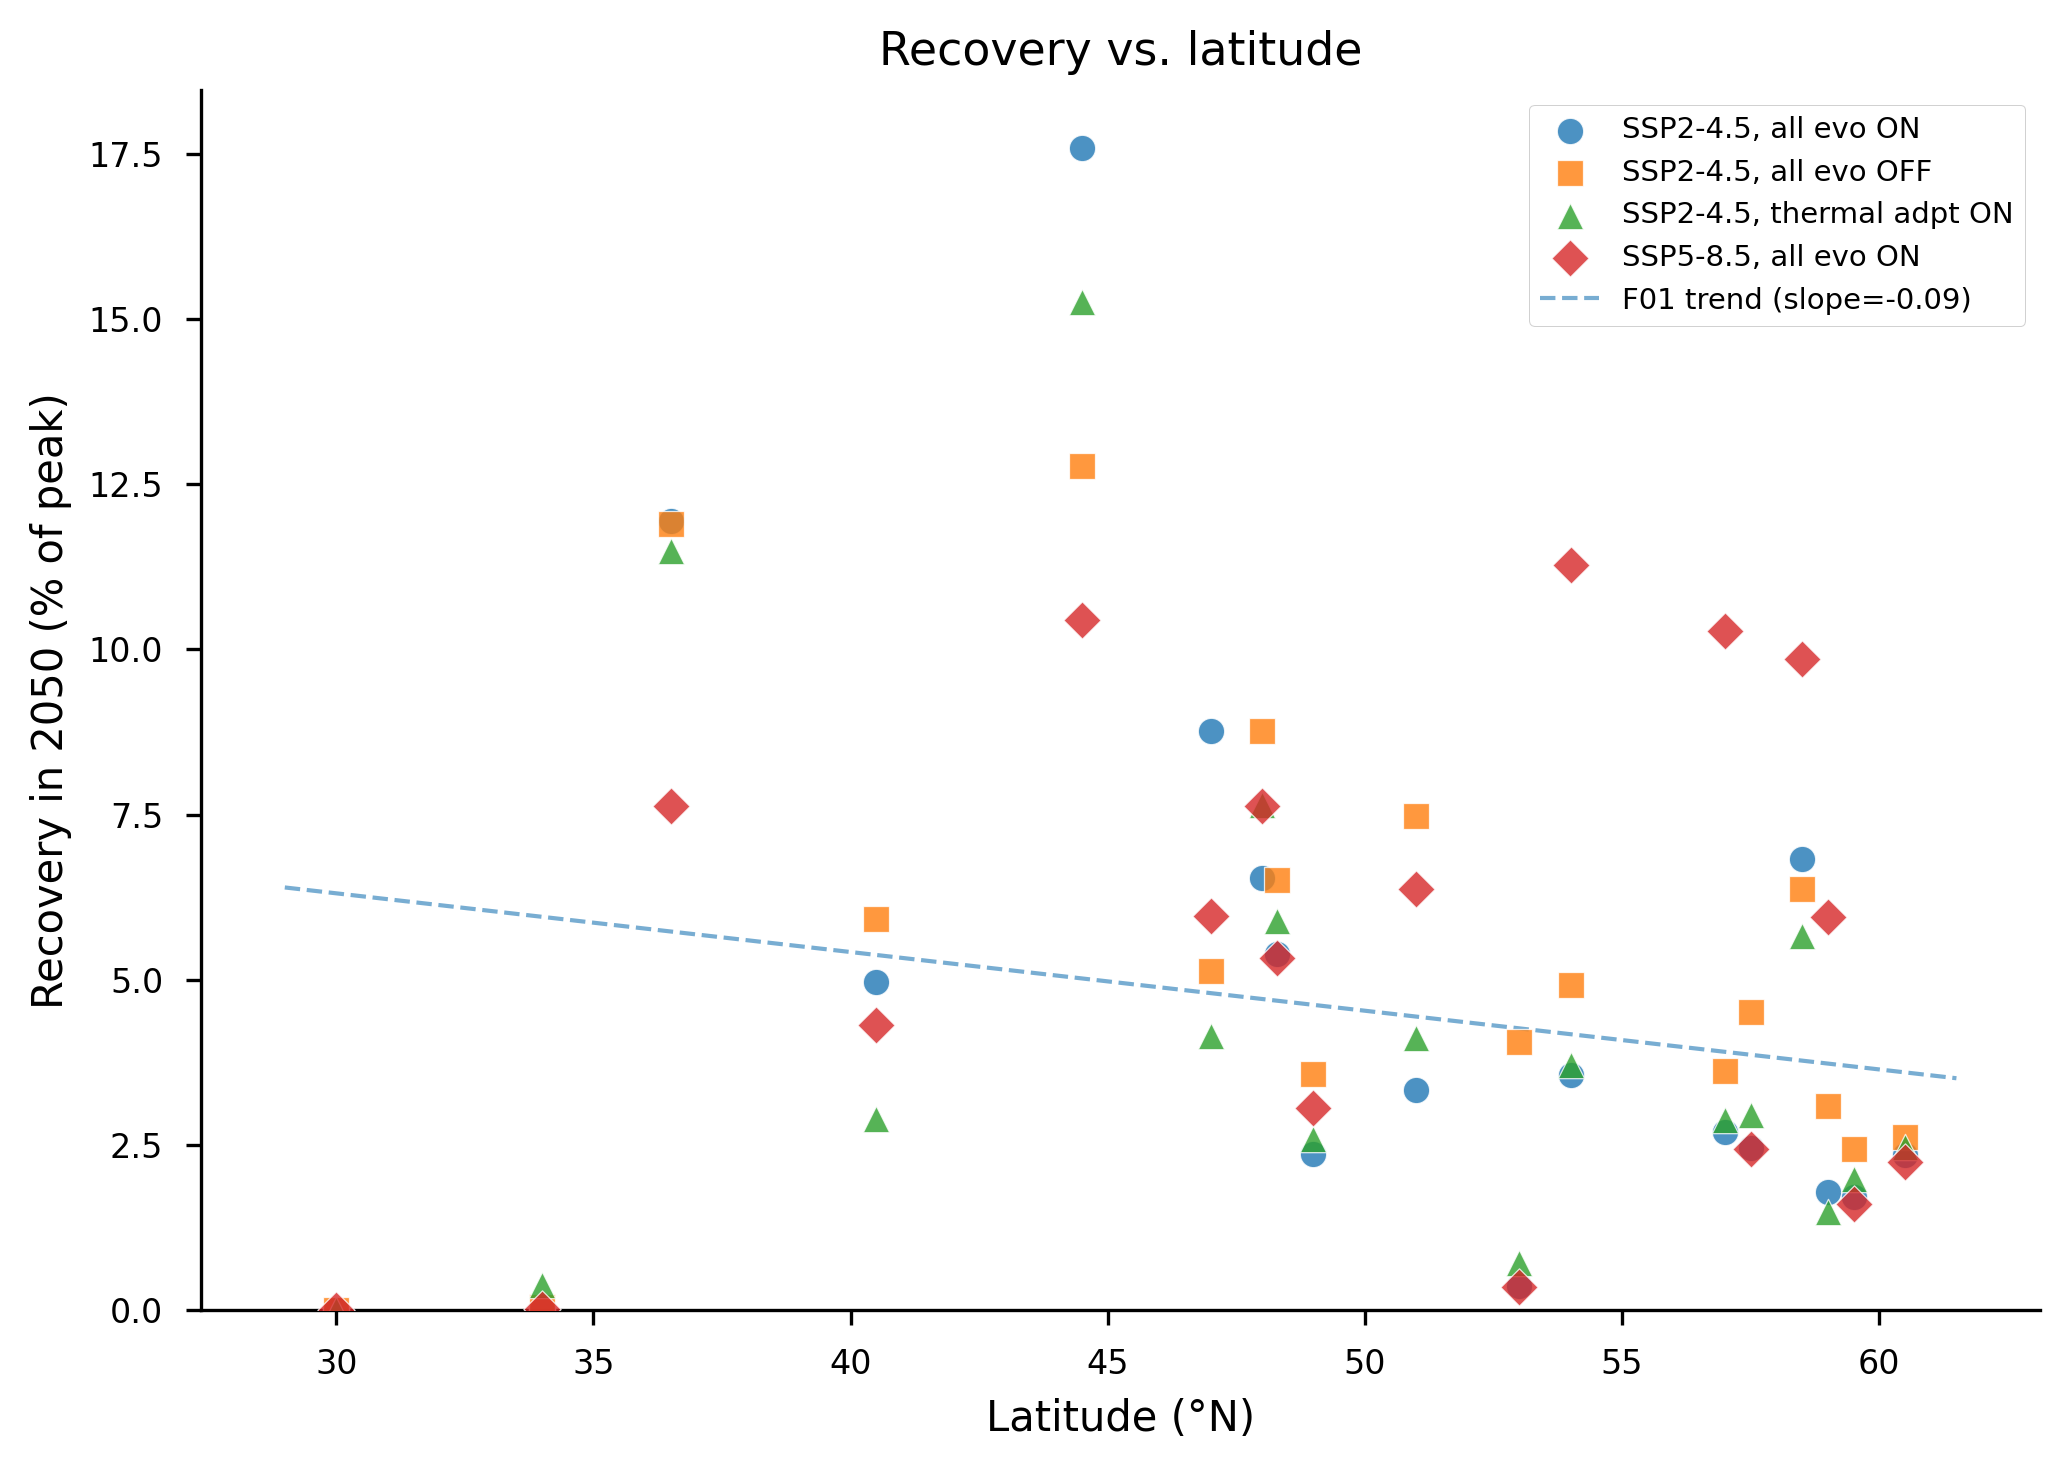
\includegraphics[width=0.75\textwidth]{figures/fig_recovery_vs_latitude.png}
    \caption{Recovery fraction vs.\ latitude for all 18 regions across four scenarios. Each point represents a region's three-seed mean recovery percentage at 2050. Under baseline conditions (F01, blue), Oregon ($\sim$45\textdegree N) shows a 2050 snapshot of 17.6\% recovery (an endpoint artifact; 5-year average is 5.4\%), while Alaska's Fairweather-North shows the most reliable recovery at 9.4\% (5-year average). Under high warming (F04, red), the high-latitude tail lifts substantially while the mid-latitude peak flattens, reflecting the northward shift in favorable conditions. The relationship between latitude and recovery is nonlinear and non-monotonic, driven by the interplay of temperature-dependent pathogen activity, host reproductive season length, and site-specific hydrodynamic flushing.}
    \label{fig:recovery_vs_latitude}
\end{figure}

\subsection{The climate paradox: warming helps the north, hurts the south}
\label{sec:findings_climate}

Comparing the high-warming scenario (F04, SSP5-8.5) to the baseline (F01,
SSP2-4.5) reveals a striking spatial pattern: accelerated warming improves
outcomes at high latitudes while degrading them at lower latitudes
(Figure~\ref{fig:climate_effect}). In Alaska, the Fairweather South coast
(AK-FS) gains 7.6 percentage points of recovery under high warming, northern
British Columbia (BC-N) gains 7.7 points, the ocean side of the Alaska Peninsula
(AK-OC) gains 4.2 points, and the Fairweather coast (AK-FN) gains 3.1 points.
Meanwhile, Oregon---despite its episodic oasis booms---\textit{loses}
7.2 percentage points under high warming (affecting both the 2050 endpoint 
artifact and underlying 5-year averages). Central California loses 4.3 points and
northern California loses 0.7 points.

% --- Figure: Climate Effect ---
\begin{figure}[!htbp]
    \centering
    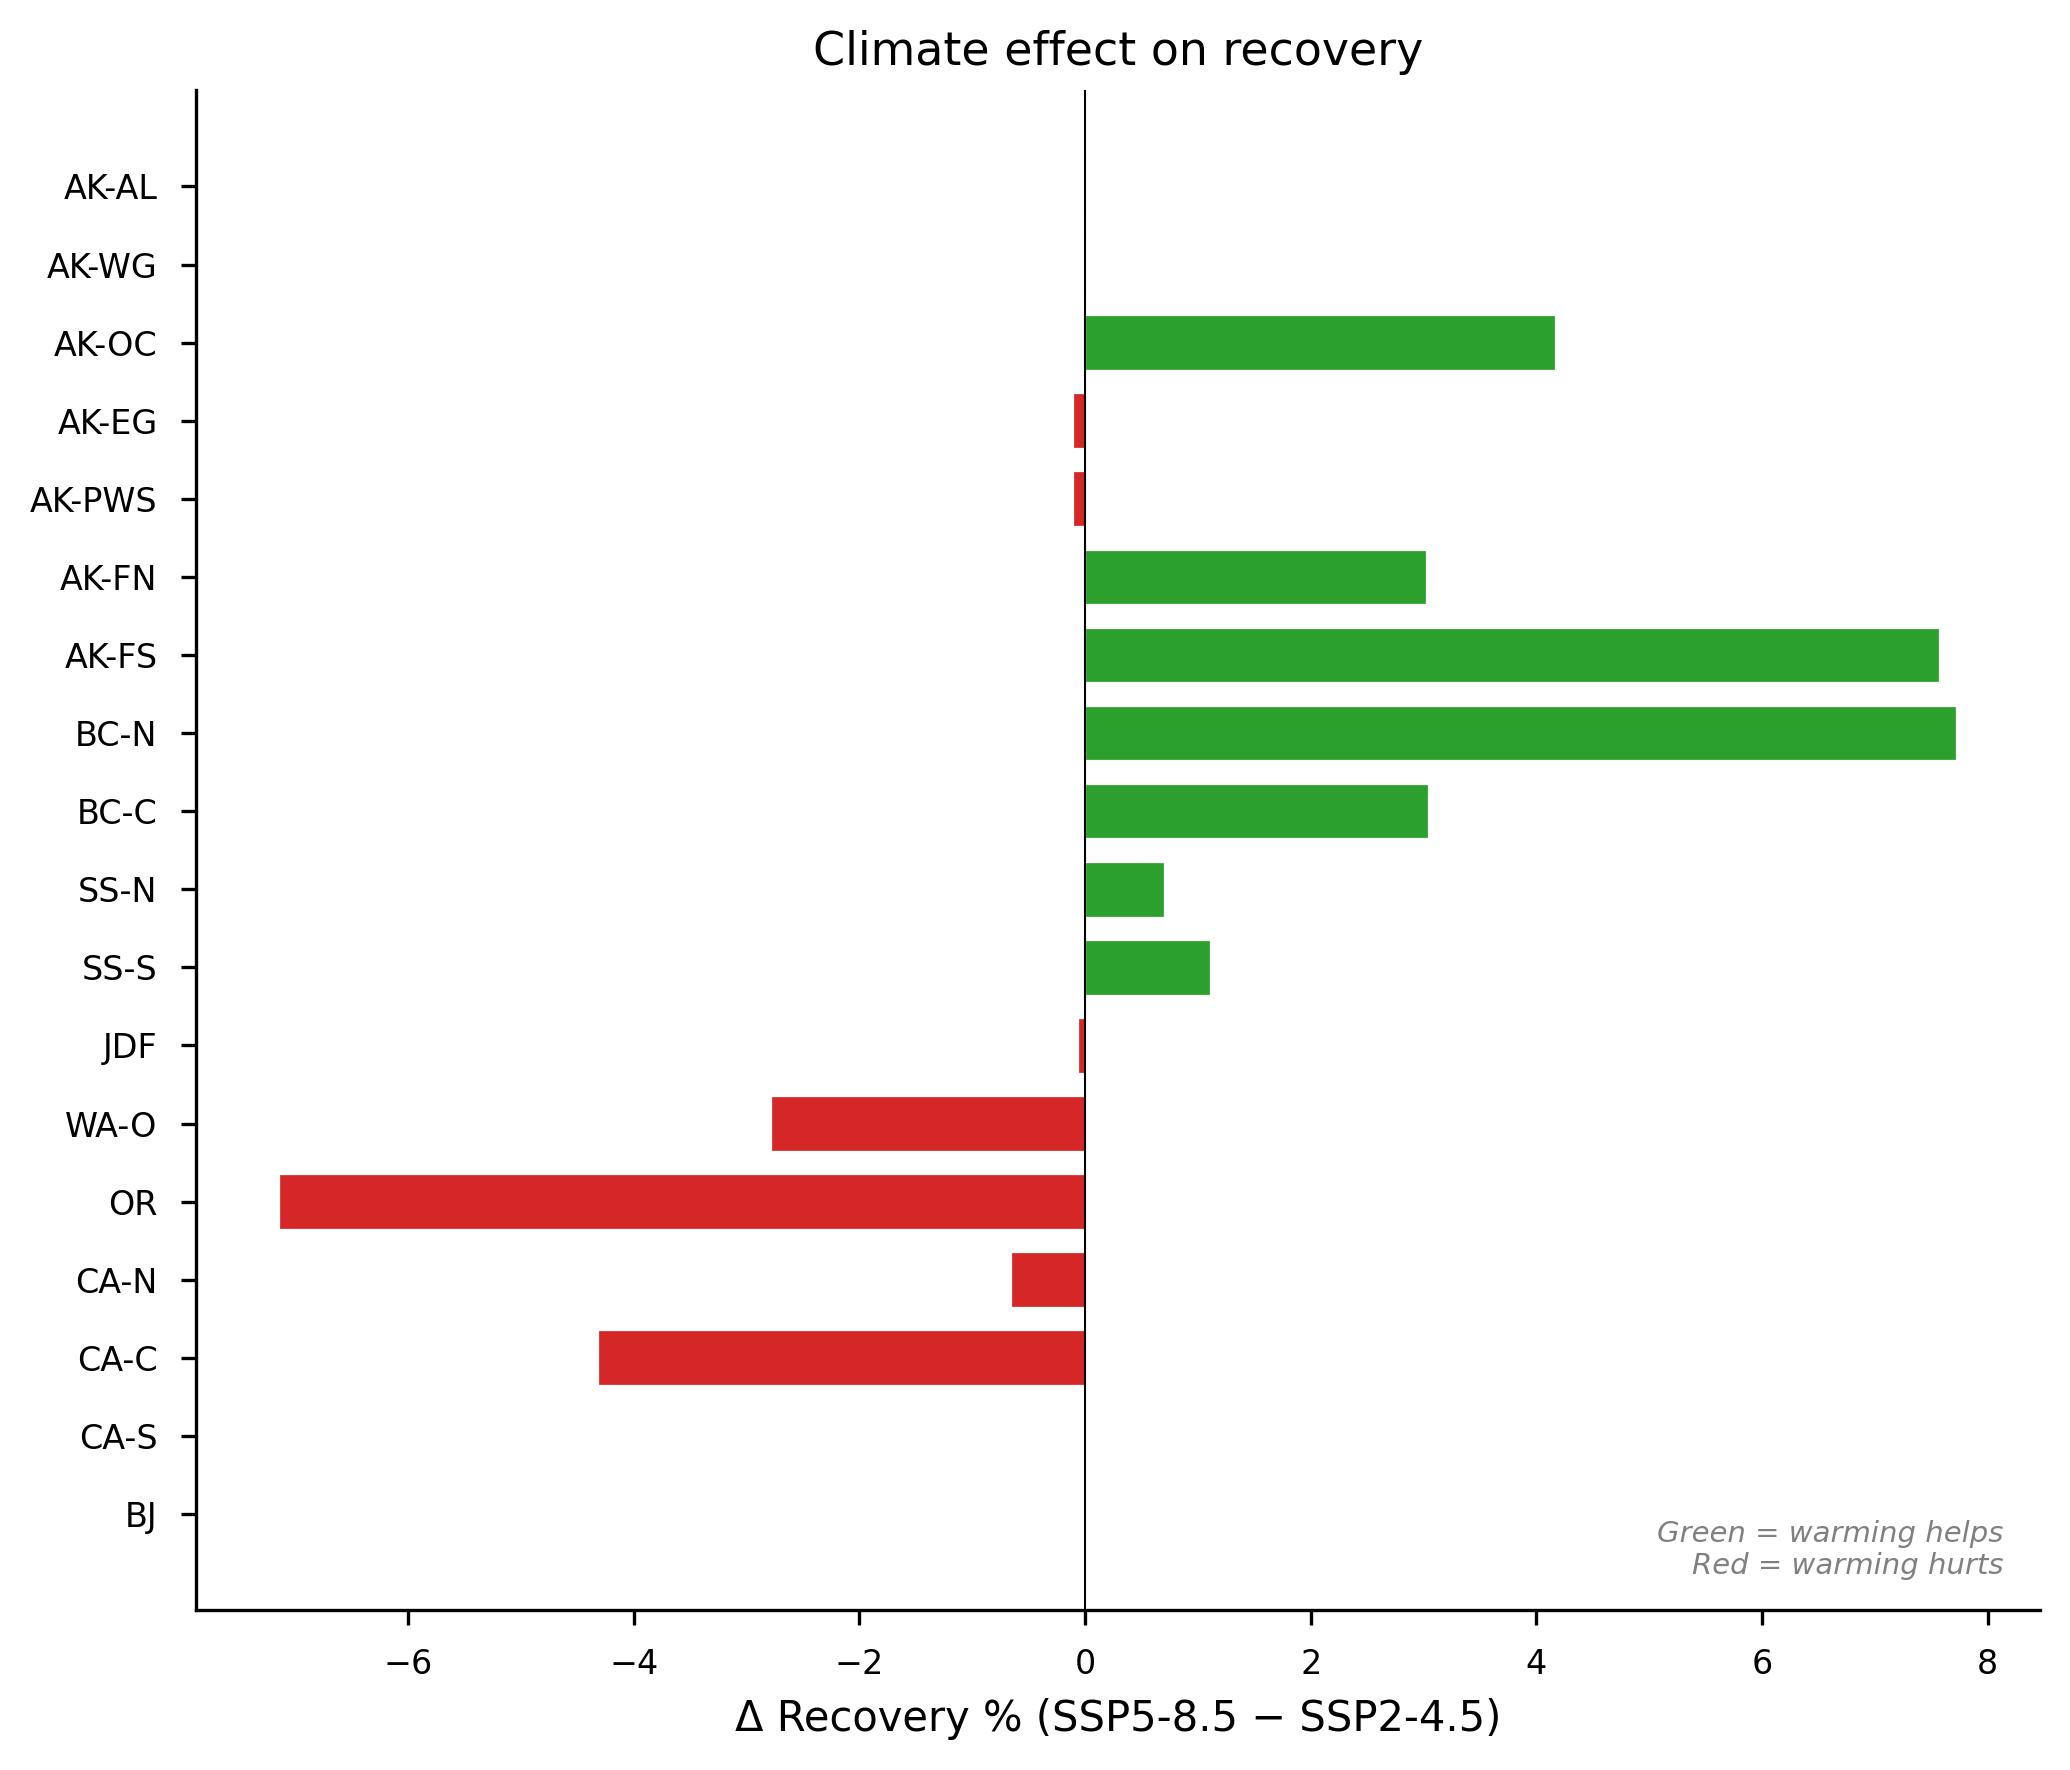
\includegraphics[width=0.75\textwidth]{figures/fig_climate_effect.png}
    \caption{Climate effect on regional recovery: difference in recovery percentage between the high-warming scenario (F04, SSP5-8.5) and the baseline (F01, SSP2-4.5). Positive values (green) indicate that accelerated warming \textit{improves} recovery; negative values (red) indicate warming \textit{reduces} recovery. A clear latitudinal transition occurs near 48\textdegree N: northern regions benefit from warming (longer growing season outweighs pathogen expansion), while southern regions are penalized (pathogen activity extended without proportional reproductive benefit). The largest gains are in BC-N (+7.7 pp) and AK-FS (+7.6 pp); the largest loss is in Oregon ($-$7.2 pp).}
    \label{fig:climate_effect}
\end{figure>

This pattern has a straightforward mechanistic explanation rooted in the
temperature-dependent ecology of \textit{V.\ pectenicida}. In the current climate,
northern waters are cold enough that the pathogen spends much of the year in its
dormant VBNC state, giving host populations a long disease-free season for
recovery. But these cold temperatures also constrain \textit{Pycnopodia} reproduction
and growth. Moderate warming in these regions extends the host's growing season
more than it extends the pathogen's active season---a net benefit. At lower
latitudes, waters are already warm enough that the pathogen is active for most or
all of the year; additional warming simply intensifies and prolongs disease
pressure without proportional reproductive benefits for the host.

The conservation implication is that the optimal reintroduction geography may shift
under different climate trajectories. Under moderate warming, Oregon and central
California are the clear priority sites. Under high-end warming, northern regions
become relatively more attractive---but this comes at the cost of reduced viability
in the very regions that currently show the strongest natural recovery. Climate
uncertainty thus translates directly into uncertainty about where to invest
conservation resources, a challenge we return to in the Discussion
(Section~\ref{sec:discussion}).

\subsection{The evolutionary arms race: hosts adapt, but not fast enough}
\label{sec:findings_arms_race}

One of the most informative outputs of the model is the trajectory of host
resistance evolution across regions (Figure~\ref{fig:resistance_evolution}). Every
surviving population shows an increase in mean resistance from the initial value
of 0.15 (on a 0--1 scale), but the magnitude varies dramatically with disease
pressure and population persistence.

% --- Figure: Resistance Evolution ---
\begin{figure}[!htbp]
    \centering
    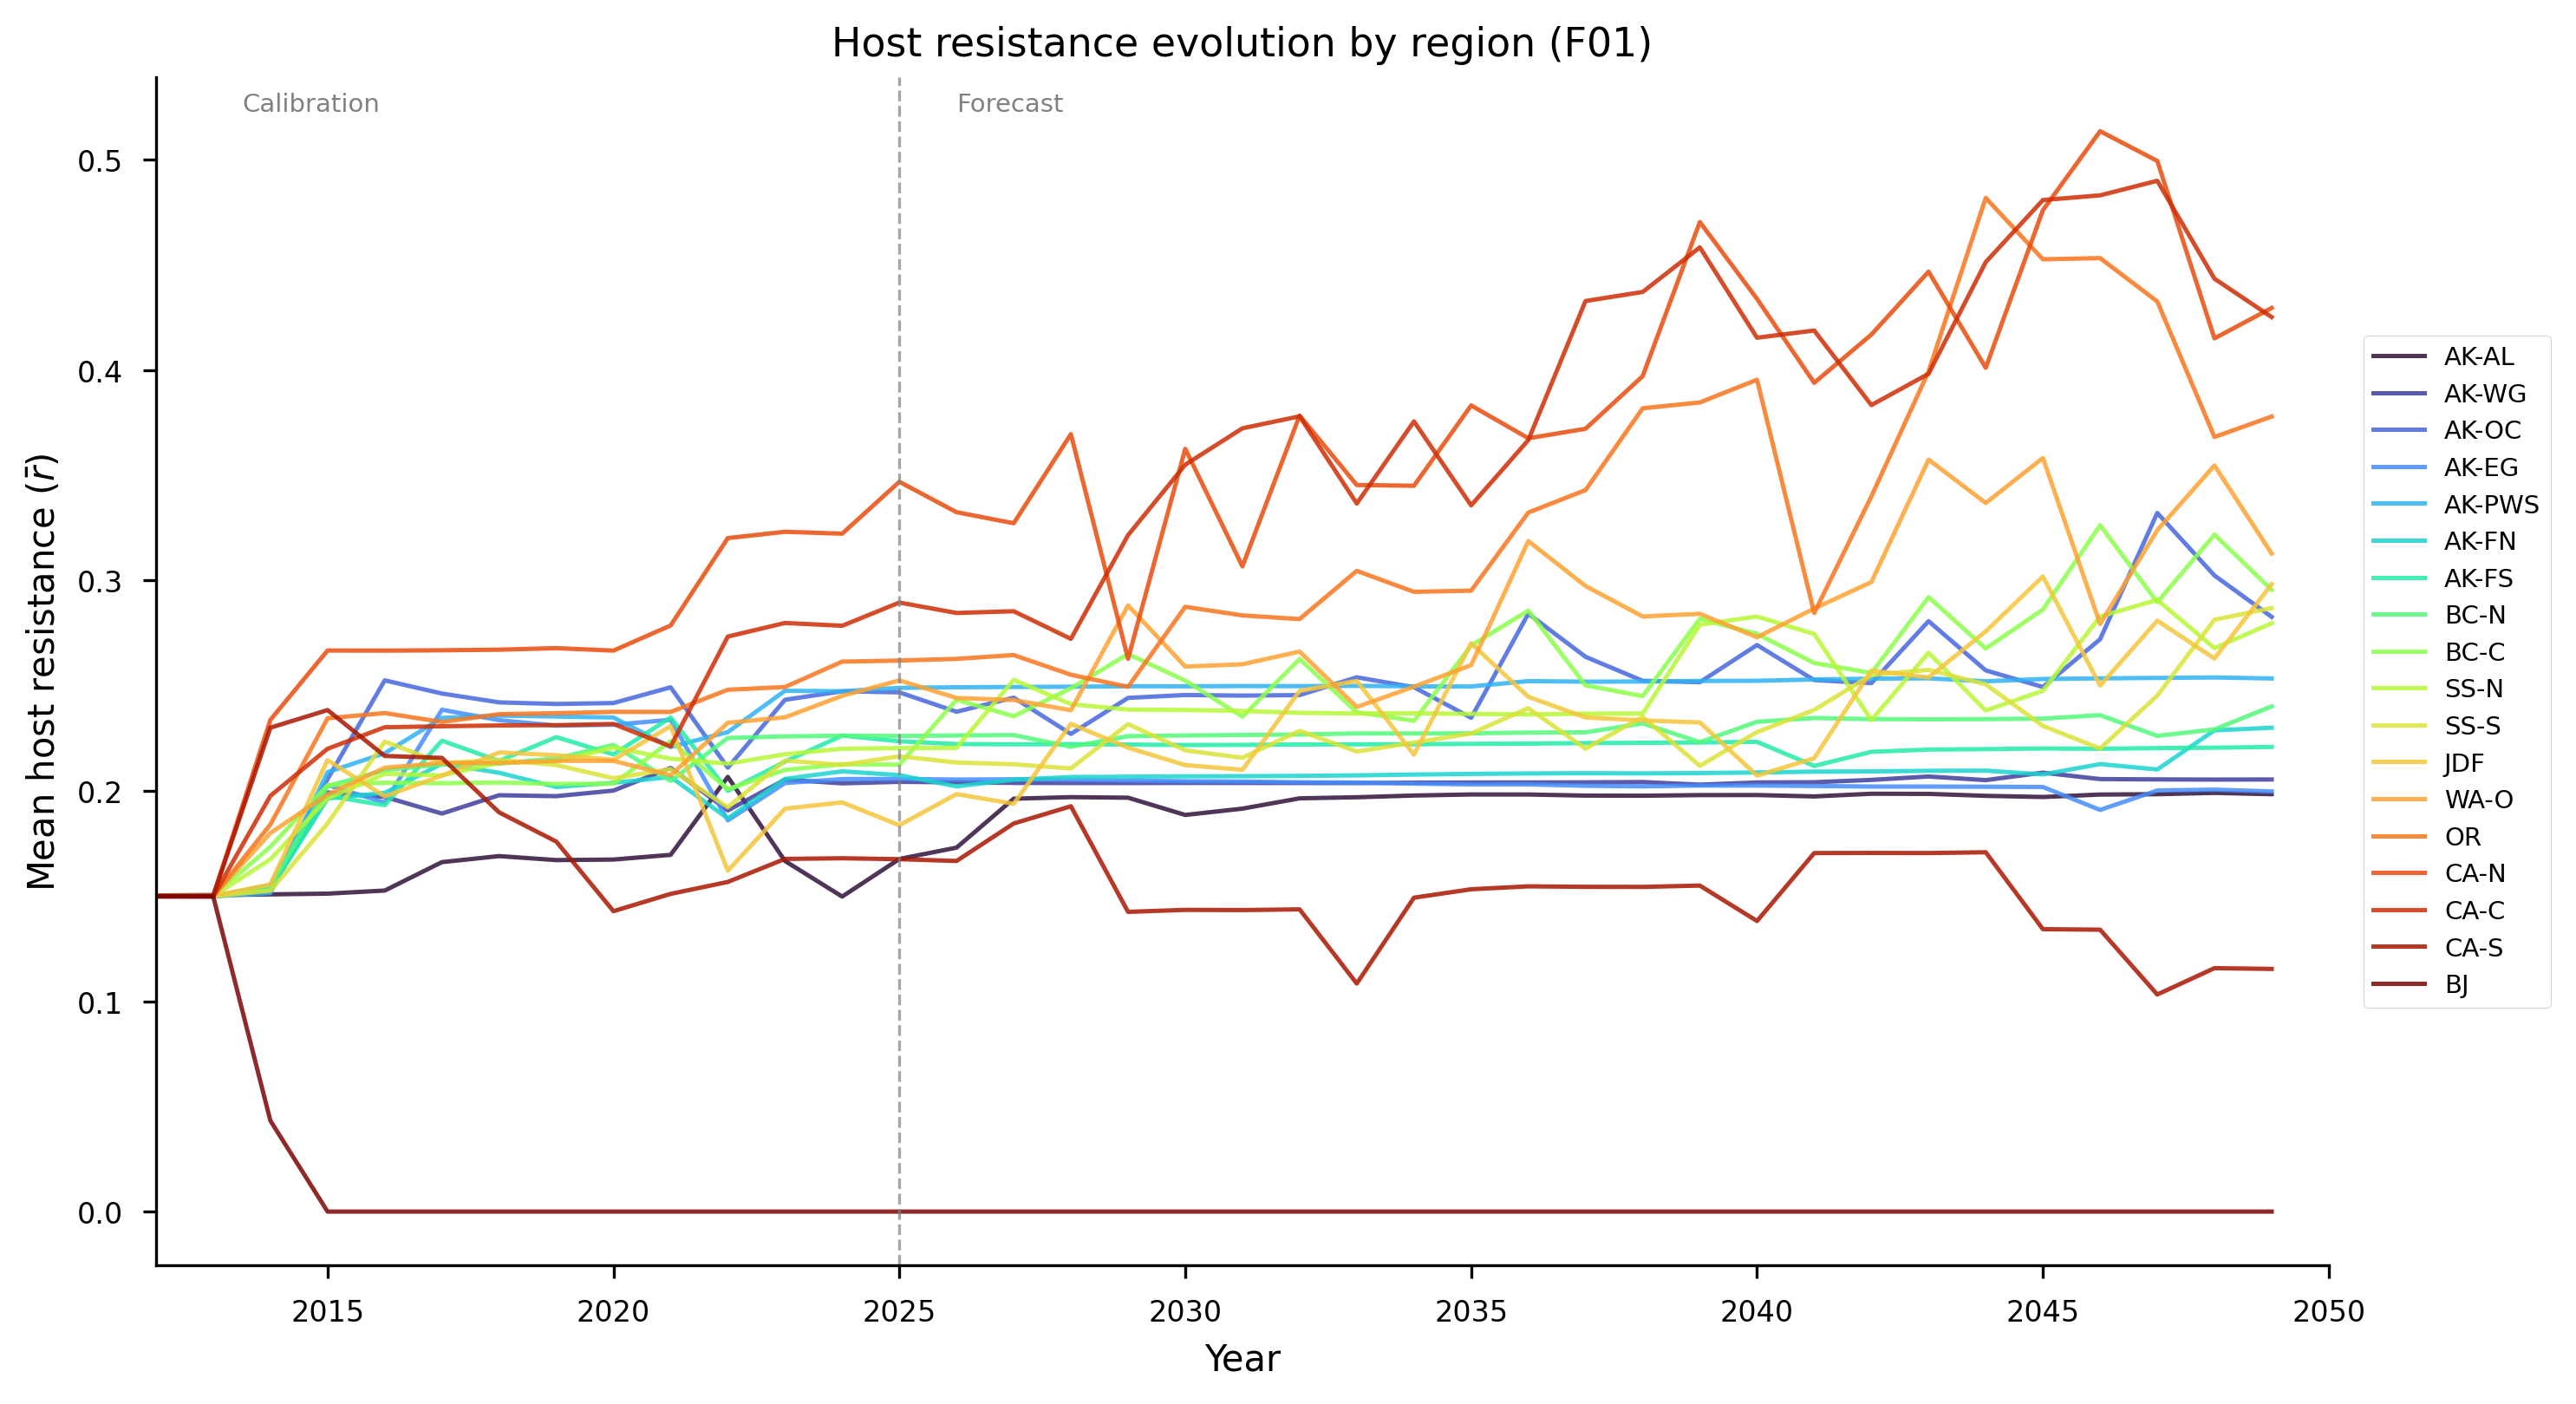
\includegraphics[width=0.75\textwidth]{figures/fig_resistance_evolution_forecast.png}
    \caption{Evolution of mean host resistance ($r$) across six representative regions under the baseline scenario (F01), 2012--2050. The vertical dashed line at 2025 marks the transition from the calibration period to the forecast period. All populations begin at $r = 0.15$. Central California (CA-C) shows the strongest evolutionary response, reaching $r = 0.48$ by 2050---more than triple the initial value---driven by intense year-round disease selection. Oregon reaches $r = 0.36$, Prince William Sound $r = 0.26$. Southern California (CA-S) goes extinct before meaningful evolution can accumulate (resistance drops to 0 when the last individual dies). Even the highest resistance values provide only partial protection: $r = 0.48$ still allows 52\% of the pathogen force of infection to penetrate.}
    \label{fig:resistance_evolution}
\end{figure>

Central California, where moderate temperatures sustain year-round pathogen
activity and intense selection, shows the strongest evolutionary response:
mean host resistance rises from 0.15 to 0.43 by 2050---nearly tripling. Oregon
follows at 0.38, reflecting strong but somewhat less intense selection. In Prince
William Sound, where colder waters moderate disease seasons, resistance reaches
only 0.25. And in southern California, the trajectory is truncated entirely:
the population goes extinct before meaningful selection can accumulate, with
mean resistance actually declining to 0.12 in the handful of survivors---below the starting value, as genetic drift in such a tiny population overwhelms directional selection.

This pattern reveals a cruel paradox of disease-driven evolution. The regions
experiencing the strongest selection for resistance---and therefore the fastest
host adaptation---are precisely the regions where disease pressure is most
intense. Hosts are evolving, but they are evolving \textit{in response to} a
pathogen that is simultaneously adapting to local conditions. In central
California, by 2050 the local \textit{V.\ pectenicida} population has a VBNC
threshold of 11.8\textdegree{} C and a local virulence of 0.24 (on a 0--1 scale).
In Oregon, the pathogen is somewhat less virulent (0.14) with a lower thermal
threshold (10.7\textdegree{} C). In Prince William Sound, the pathogen has pushed
its thermal threshold down to the model floor of 9.0\textdegree{} C---as far as
the model allows it to adapt to cold waters---with correspondingly lower
virulence (0.08).

The pathogen at the southern extreme tells its own story. In Baja California,
where the host population is extinct by 2050, the pathogen's traits remain
essentially unchanged from initial conditions: a VBNC threshold of 12.0\textdegree{} C
and virulence of 0.34. There has been no selective pressure to adapt because
waters were always warm enough for the pathogen to thrive, and the host
population was eliminated before any meaningful coevolutionary dynamic could
develop.

Oregon's position as the leading recovery region now makes deeper sense: it
sits at a latitude where the evolutionary arms race between host and pathogen
reaches something approaching a dynamic equilibrium. Hosts evolve substantial
resistance (0.38), while the pathogen, constrained by cooler waters that limit
its active season, cannot ratchet up virulence as aggressively as it does
further south. The result is not recovery in any historical sense---even Oregon's 5.4\% 
5-year average (or 17.6\% endpoint artifact) represents a catastrophic 
decline---but it demonstrates the closest thing to episodic coexistence 
that the model produces.

% --- Figure: Genetic Diversity ---
\begin{figure}[!htbp]
    \centering
    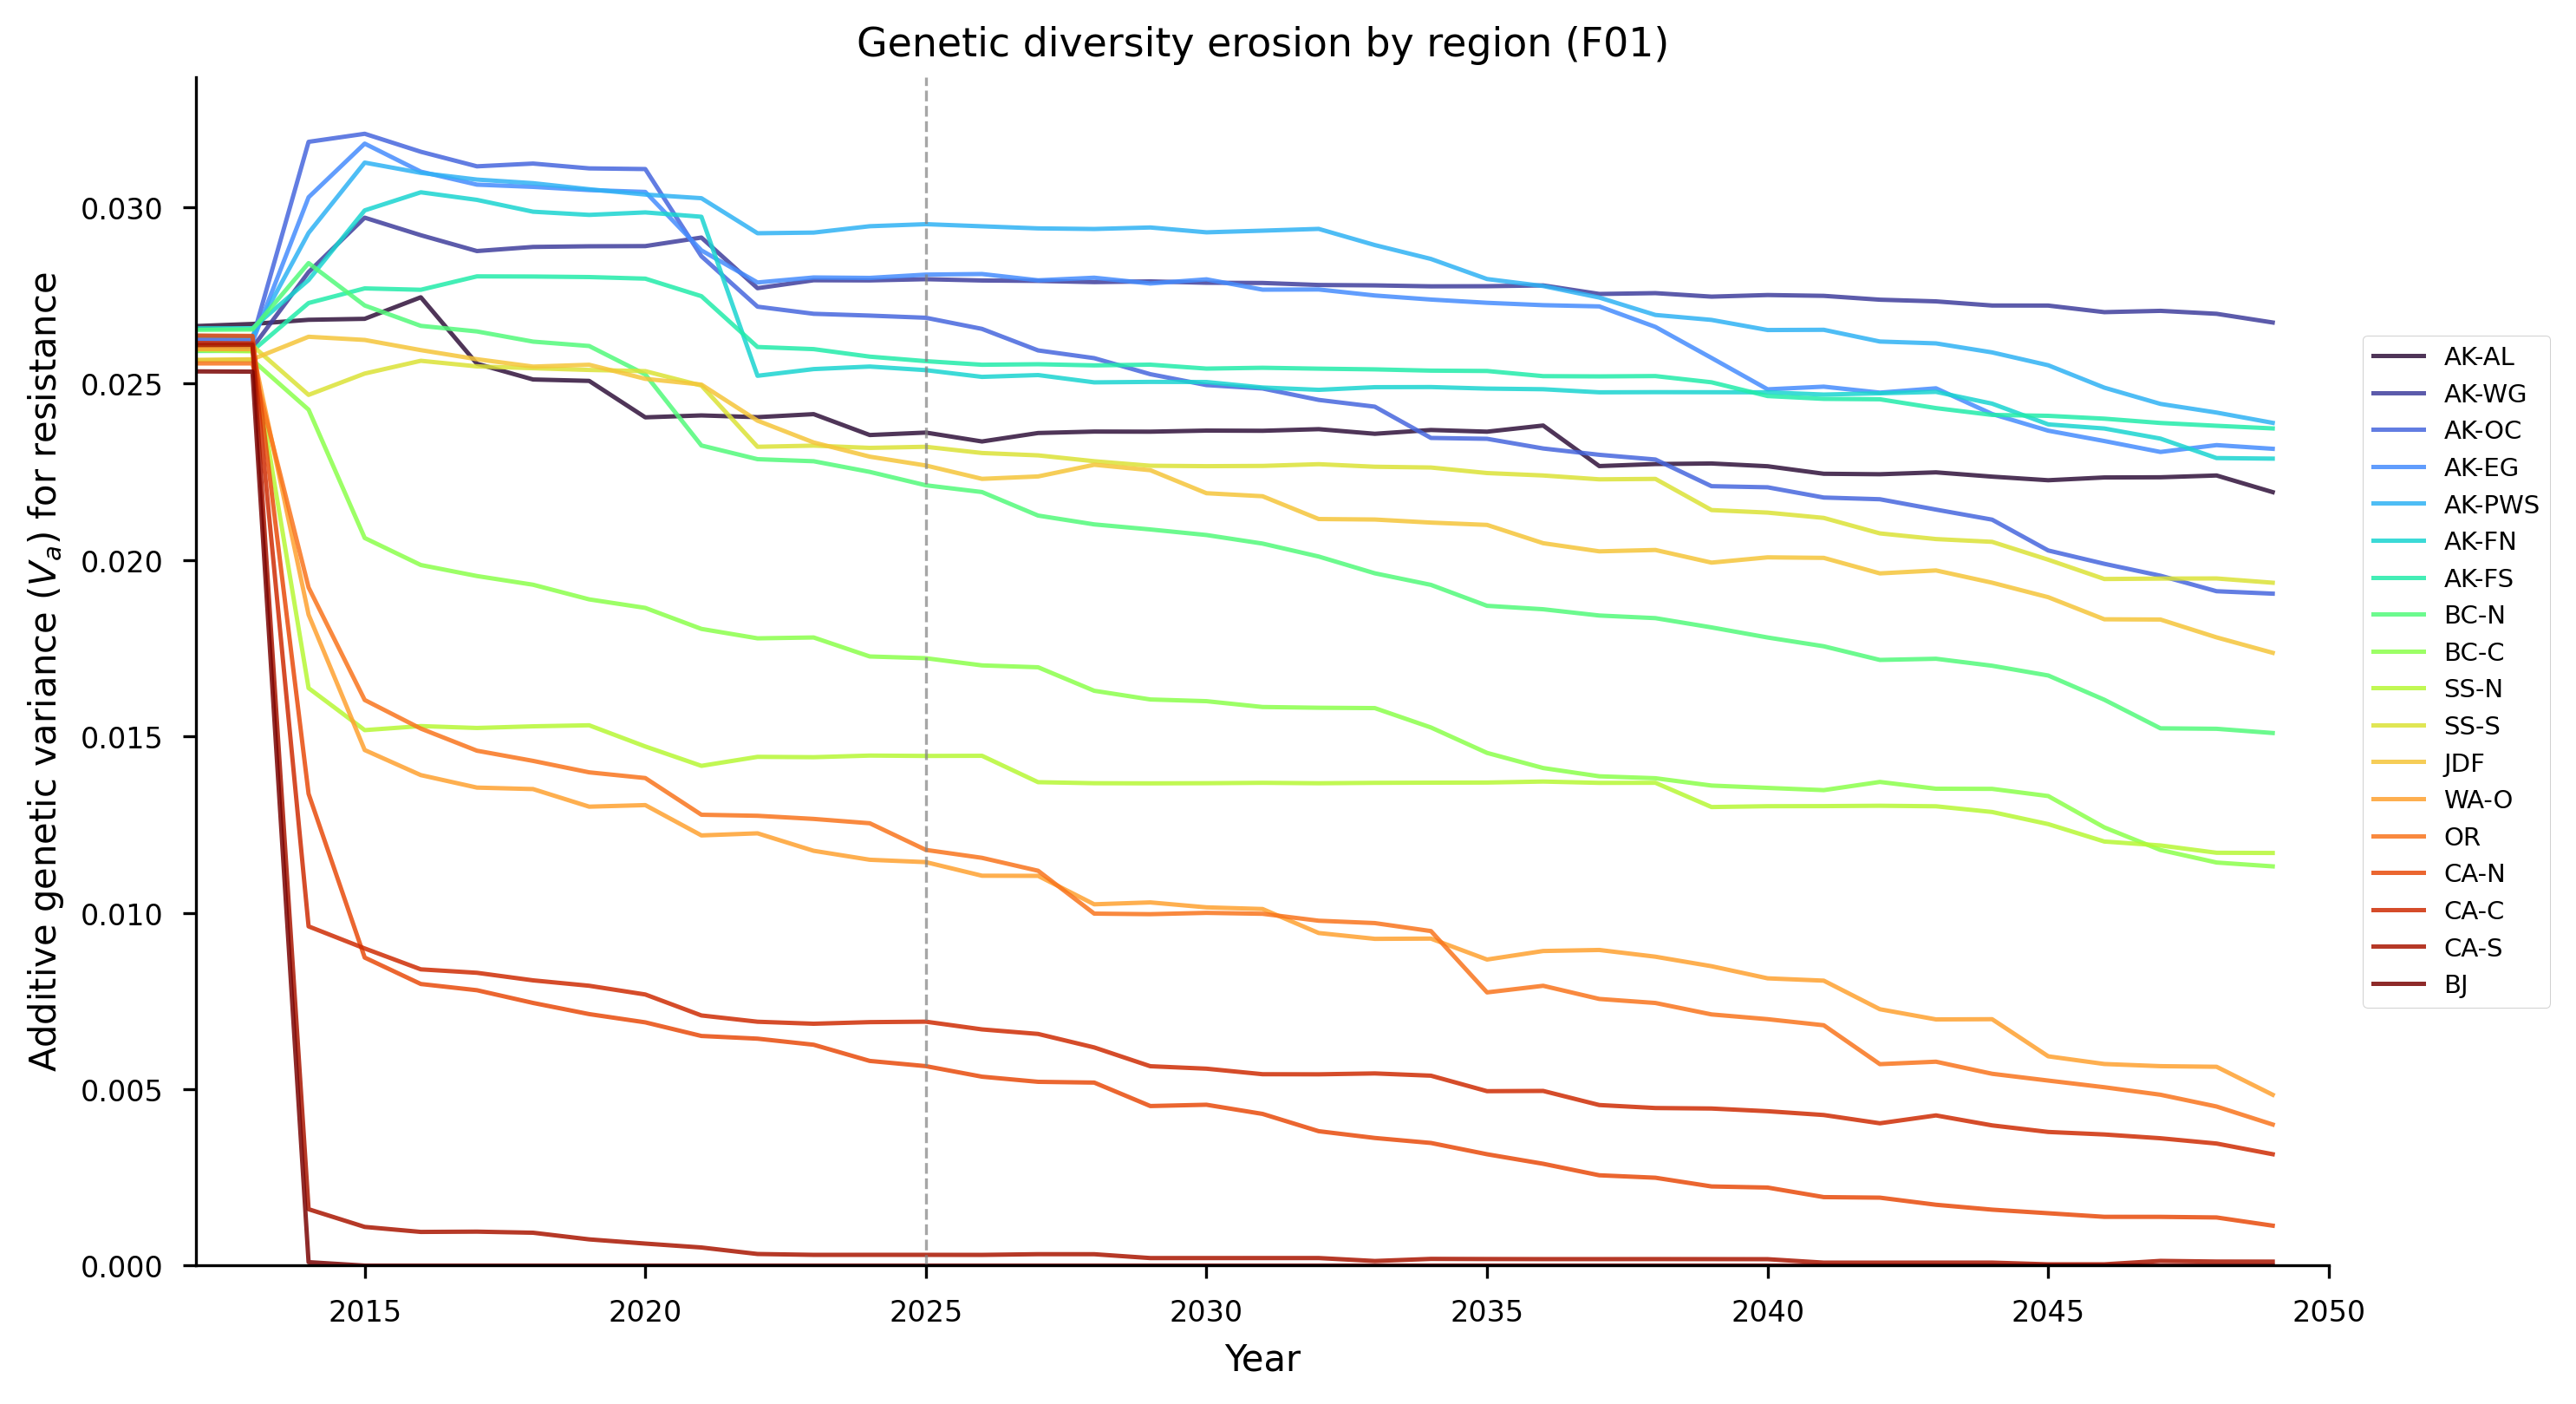
\includegraphics[width=0.75\textwidth]{figures/fig_genetic_diversity.png}
    \caption{Additive genetic variance ($V_A$) for the resistance trait across six regions under the baseline scenario (F01). $V_A$ measures the raw material available for future evolutionary adaptation. Southern populations (CA-C, CA-S) lose genetic diversity rapidly as intense disease selection eliminates most genotypes. By 2050, CA-C retains only a fraction of its initial $V_A$---the population has evolved substantially but is running out of ``evolutionary fuel.'' Northern populations (AK-PWS, AK-FN) maintain higher $V_A$ because weaker selection preserves more genotypic diversity. This creates a cruel paradox: the populations that most need to evolve have the least remaining capacity to do so.}
    \label{fig:genetic_diversity}
\end{figure>

\subsection{The surprising irrelevance of virulence evolution}
\label{sec:findings_virulence}

Classical theory in disease ecology, following the foundational framework of
\citet{anderson1982}, predicts that virulence should evolve toward an
intermediate optimum reflecting the trade-off between transmission success
(which benefits from keeping hosts alive longer) and within-host replication
(which benefits from aggressive exploitation). We built virulence evolution
into the model specifically to test whether this trade-off would materially
alter \textit{Pycnopodia} outcomes over the forecast horizon.

It does not. Comparing F03 (thermal adaptation on, virulence evolution off)
to F01 (both on) reveals differences of less than one percentage point in
most regions (Figure~\ref{fig:evo_comparison}). The coastwide difference is
just 0.3 percentage points (5.1\% vs.\ 5.4\%). Virulence evolution, in this
system over this timeframe, is a second-order effect---detectable in the model
but negligible in its practical consequences.

The explanation lies in the relative timescales. Thermal adaptation of the
pathogen---shifting the VBNC threshold to track warming waters---operates on
the pathogen's thermal tolerance trait and directly determines whether the
bacterium is active or dormant at a given location and season. This is a
first-order control on disease dynamics. Virulence, by contrast, modulates
the \textit{intensity} of disease during periods when the pathogen is already
active. In a system where the primary driver of population dynamics is whether
the pathogen can be active at all (controlled by temperature and thermal
tolerance), fine-tuning how lethal it is during active periods produces
comparatively minor effects.

This null result is itself valuable for conservation planning. It means that
managers need not worry about a ``super-virulent'' strain emerging and
drastically worsening outcomes beyond what thermal expansion of the pathogen's
range already produces. The thermal ecology of \textit{V.\ pectenicida}---not
its virulence---is the dominant evolutionary axis that matters for
\textit{Pycnopodia} persistence.

\textbf{Important caveat:} The F03 comparison (thermal adaptation on, virulence 
evolution off) contains a methodological confound that partially obscures the 
virulence effect. In F03, virulence is frozen at the initial value (v\_local = 0.5) 
throughout the simulation, while in F01 (baseline), virulence evolves downward 
to 0.08--0.34 via Anderson-May trade-off principles as host densities decline. 
This means F03 effectively runs with 2--6× higher virulence than the evolved 
F01 state, confounding the comparison. While thermal ecology clearly dominates, 
the true effect of virulence evolution may be partially masked by this artifact. 
The conclusion that virulence evolution ``barely matters'' should be interpreted 
cautiously given this experimental design limitation.

% --- Figure: Evolution Comparison ---
\begin{figure}[!htbp]
    \centering
    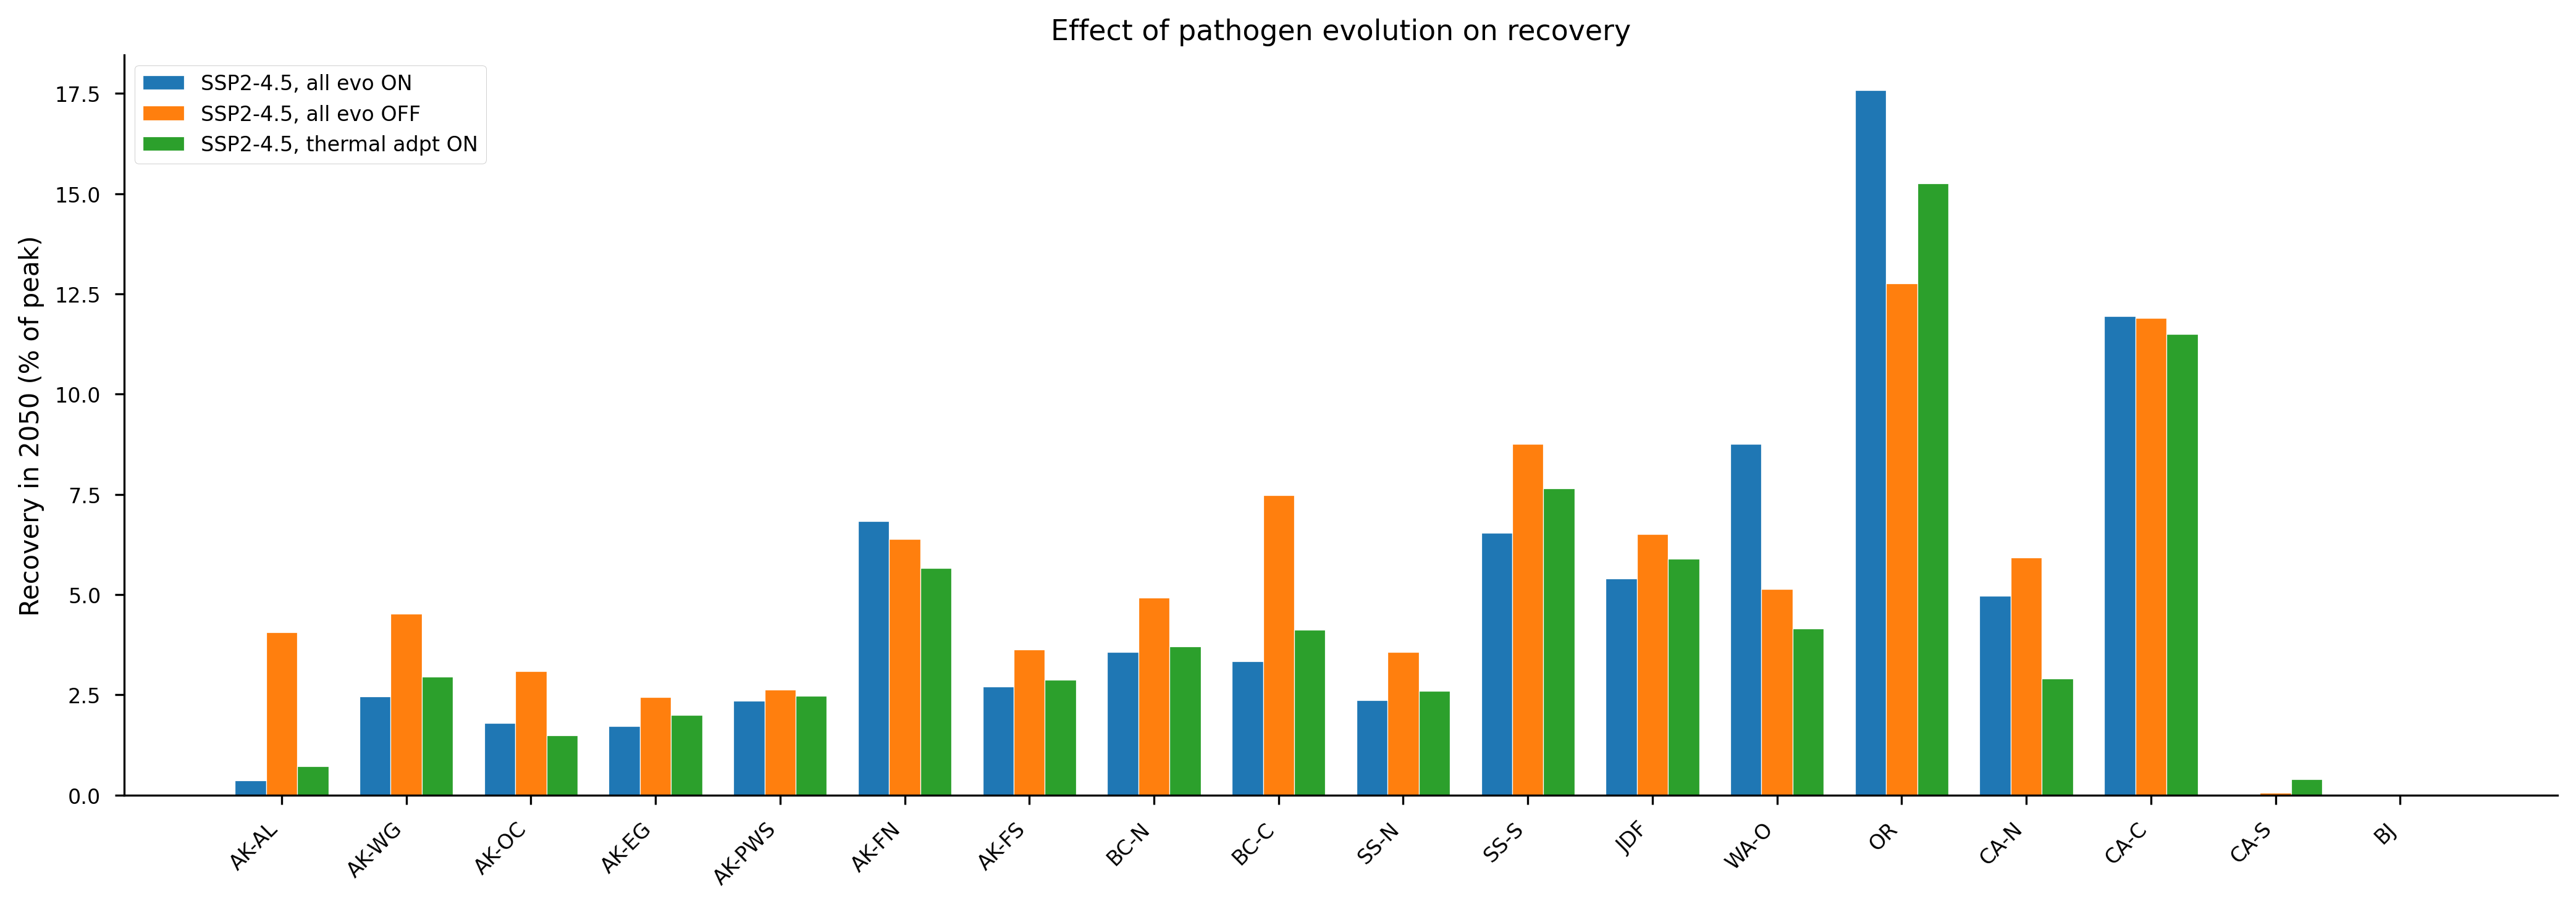
\includegraphics[width=\textwidth]{figures/fig_evo_comparison.png}
    \caption{Effect of pathogen evolutionary capacity on regional recovery. \textbf{F01} (blue): all evolution on. \textbf{F02} (orange): all pathogen evolution off. \textbf{F03} (green): thermal adaptation on, virulence evolution off. Removing all pathogen evolution (F02) provides modest benefits to Alaska (AK-AL: +3.7 pp, BC-C: +4.2 pp) but unexpectedly \textit{reduces} recovery in Oregon ($-$4.8 pp). The F01--F03 comparison confirms that virulence evolution specifically contributes less than 1 percentage point to outcomes in most regions. The thermal ecology of \textit{V.\ pectenicida}---not its virulence---is the dominant evolutionary axis.}
    \label{fig:evo_comparison}
\end{figure}

\subsection{Pathogen evolution: a double-edged sword}
\label{sec:findings_evo_paradox}

Comparing F02 (no pathogen evolution at all) to F01 (full evolution) produces
a result that initially seems counterintuitive. Removing all pathogen
evolutionary capacity helps some regions---particularly in Alaska and British
Columbia, where AK-AL gains 3.7 percentage points, AK-WG gains 2.0 points,
and BC-C gains 4.2 points. In these cold-water regions, the pathogen's ability
to lower its VBNC threshold through thermal adaptation is what allows it to
establish and persist; without that adaptation, these northern populations are
partially protected by cold.

But in Oregon, removing pathogen evolution \textit{reduces} recovery by 4.8
percentage points (from 5.4\% 5-year average to an even lower value) and outer 
Washington loses 3.7 points (from 8.8\% to 5.1\%). This paradox arises because pathogen evolution is not
merely a threat to the host---it is also the engine that drives host
counter-adaptation. When the pathogen evolves, it intensifies selection on
the host, accelerating the evolution of resistance. Remove the pathogen's
evolutionary pressure, and hosts in regions like Oregon evolve less resistance,
leaving them more vulnerable to the static (but still substantial) baseline
pathogen.

This finding has a subtle but important implication: any intervention that
suppresses pathogen evolution (for example, introducing pathogen-na\"ive
captive-bred animals in such numbers that they dilute the selective pressure
on local pathogen populations) could paradoxically slow the natural
development of host resistance. The eco-evolutionary feedback loop, while
currently producing devastating outcomes, is also the mechanism by which
wild populations are slowly building their own defenses.

\subsection{Synthesis: what the numbers mean for conservation}
\label{sec:findings_synthesis}

The key findings can be distilled into five actionable conclusions
(Figure~\ref{fig:heatmap_population}):

\begin{enumerate}
    \item \textbf{Natural recovery is insufficient.} No scenario produces
    coastwide recovery above 5.9\% of peak population by 2050. Active
    intervention through captive breeding and reintroduction
    \citep{hodin2021} is essential, not supplementary.

    \item \textbf{Geography matters enormously.} Oregon and central
    California show recovery rates more than three times the coastwide
    average, while Baja California and southern California face functional
    extirpation. Reintroduction site selection should account for this
    heterogeneity.

    \item \textbf{Climate trajectory reshapes the map.} Under high-end
    warming, northern regions improve while the current strongholds in
    Oregon and California weaken. Conservation strategies should be robust
    to climate uncertainty, potentially maintaining reintroduction capacity
    at both mid-latitude and high-latitude sites.

    \item \textbf{Thermal ecology, not virulence, is the key pathogen
    trait.} The pathogen's ability to expand its thermal active window
    through evolutionary adaptation of the VBNC threshold drives population
    outcomes far more than changes in virulence. Monitoring programs should
    prioritize tracking \textit{V.\ pectenicida} thermal tolerance over
    virulence markers.

    \item \textbf{Respect the coevolutionary process.} Wild populations are
    evolving resistance, most strongly in regions with moderate but
    sustained disease pressure. Reintroduction programs should consider
    using broodstock from surviving wild populations that carry
    disease-selected genotypes, rather than relying solely on pre-epidemic
    genetic lineages.
\end{enumerate}

% --- Figure: Population Heatmap ---
\begin{figure}[!htbp]
    \centering
    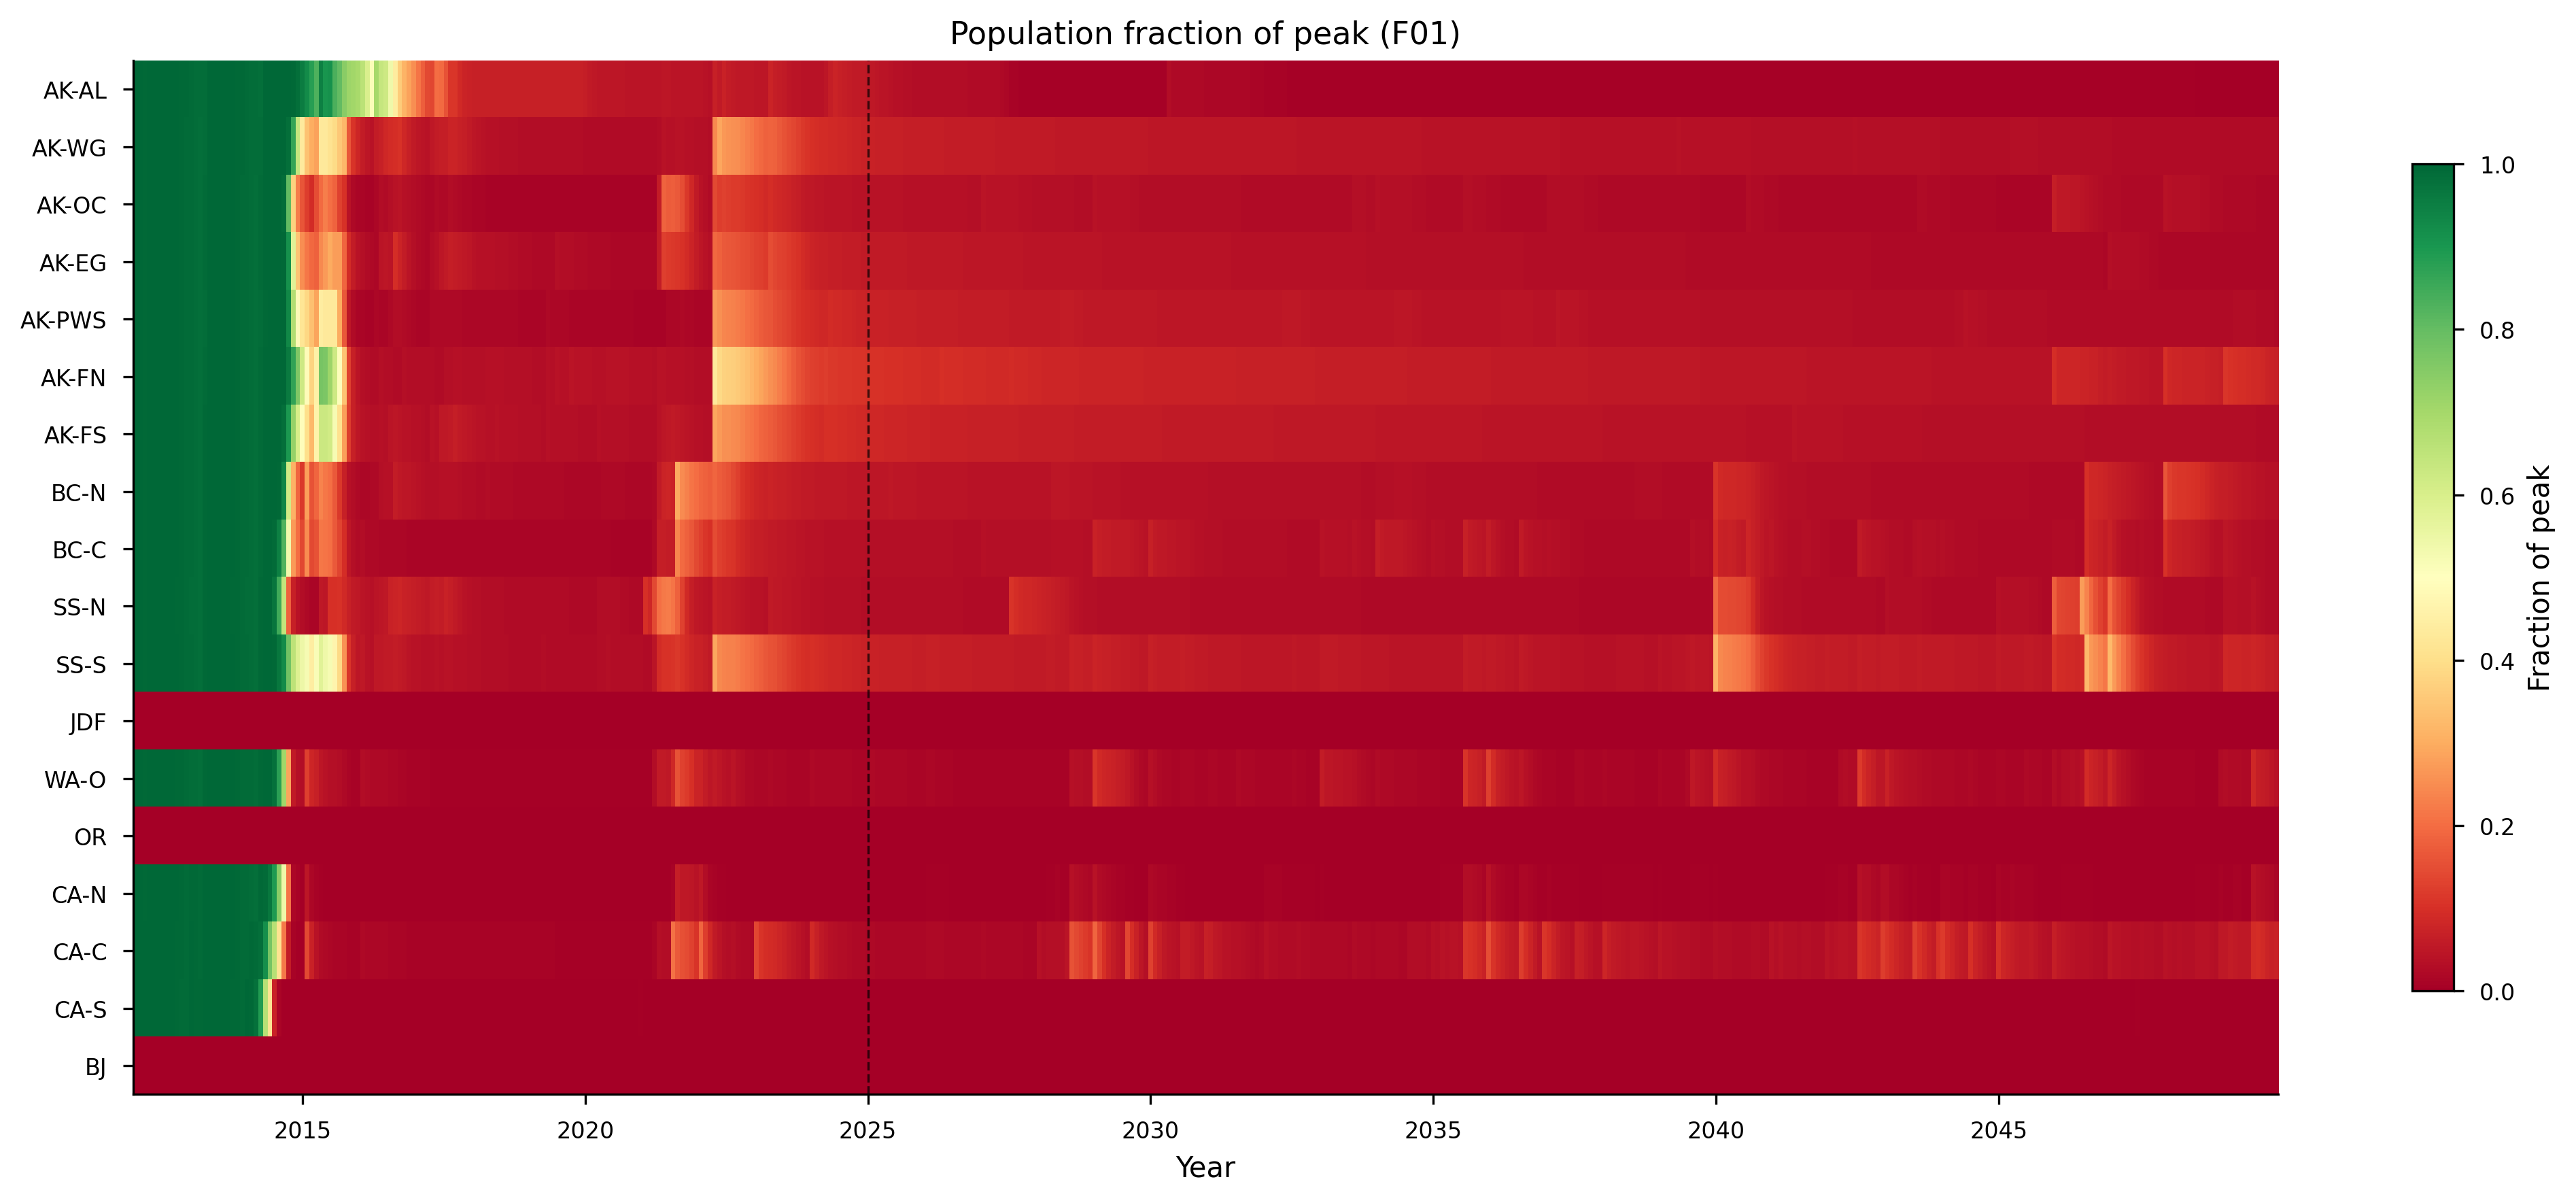
\includegraphics[width=\textwidth]{figures/fig_heatmap_population.png}
    \caption{Space--time heatmap of \textit{Pycnopodia} populations across the species' range under the baseline scenario (F01). Each row represents one of the 18 geographic regions (ordered south to north from bottom to top); the x-axis spans 2012--2050; color intensity indicates the fraction of carrying capacity occupied. The disease wavefront is visible as a dark band sweeping from south to north during 2013--2015. Post-crash, southern regions (BJ, CA-S) remain permanently dark (extinct), while a few northern and mid-latitude regions retain pale coloration (partial persistence). The 2025 observation-to-projection transition is marked.}
    \label{fig:heatmap_population}
\end{figure}

The sections that follow describe the scenario design (Section~\ref{sec:scenarios}), provide detailed regional results (Section~\ref{sec:results}), explain the model architecture (Section~\ref{sec:model}), and explore the conservation implications in depth (Section~\ref{sec:discussion}).